The author deployed the new PC RoIB in the ATLAS trigger and data acquisition 
system during the LHC winter shutdown in January 2016. 
Initially, the PC RoIB was used as the main system with the VMEbus RoIB 
was used as a backup system. Later, the VMEbus RoIB was removed completely
and the PC RoIB became the only system running in the ATLAS trigger.
The PC RoIB operated reliably since its installation without any problems 
and without deadtime for the ATLAS data collection. 
Figure \ref{fig:roib.perf.buildtime} shows that
the RoIB event assembly does not depend on pileup conditions and
Figure \ref{fig:roib.perf.mem} shows that the 
memory usage of the HLTSV is at the level of 5\%.
It has now participated in collecting a dataset of over  35 \ifb exceeding 
the dataset collected by the VMEbus RoIB (22 \ifb).
The performance of the PC RoIB during the data taking of ATLAS has been 
very stable.



\begin{figure}[t!]
\centering
\begin{subfigure}[t]{0.48\textwidth}
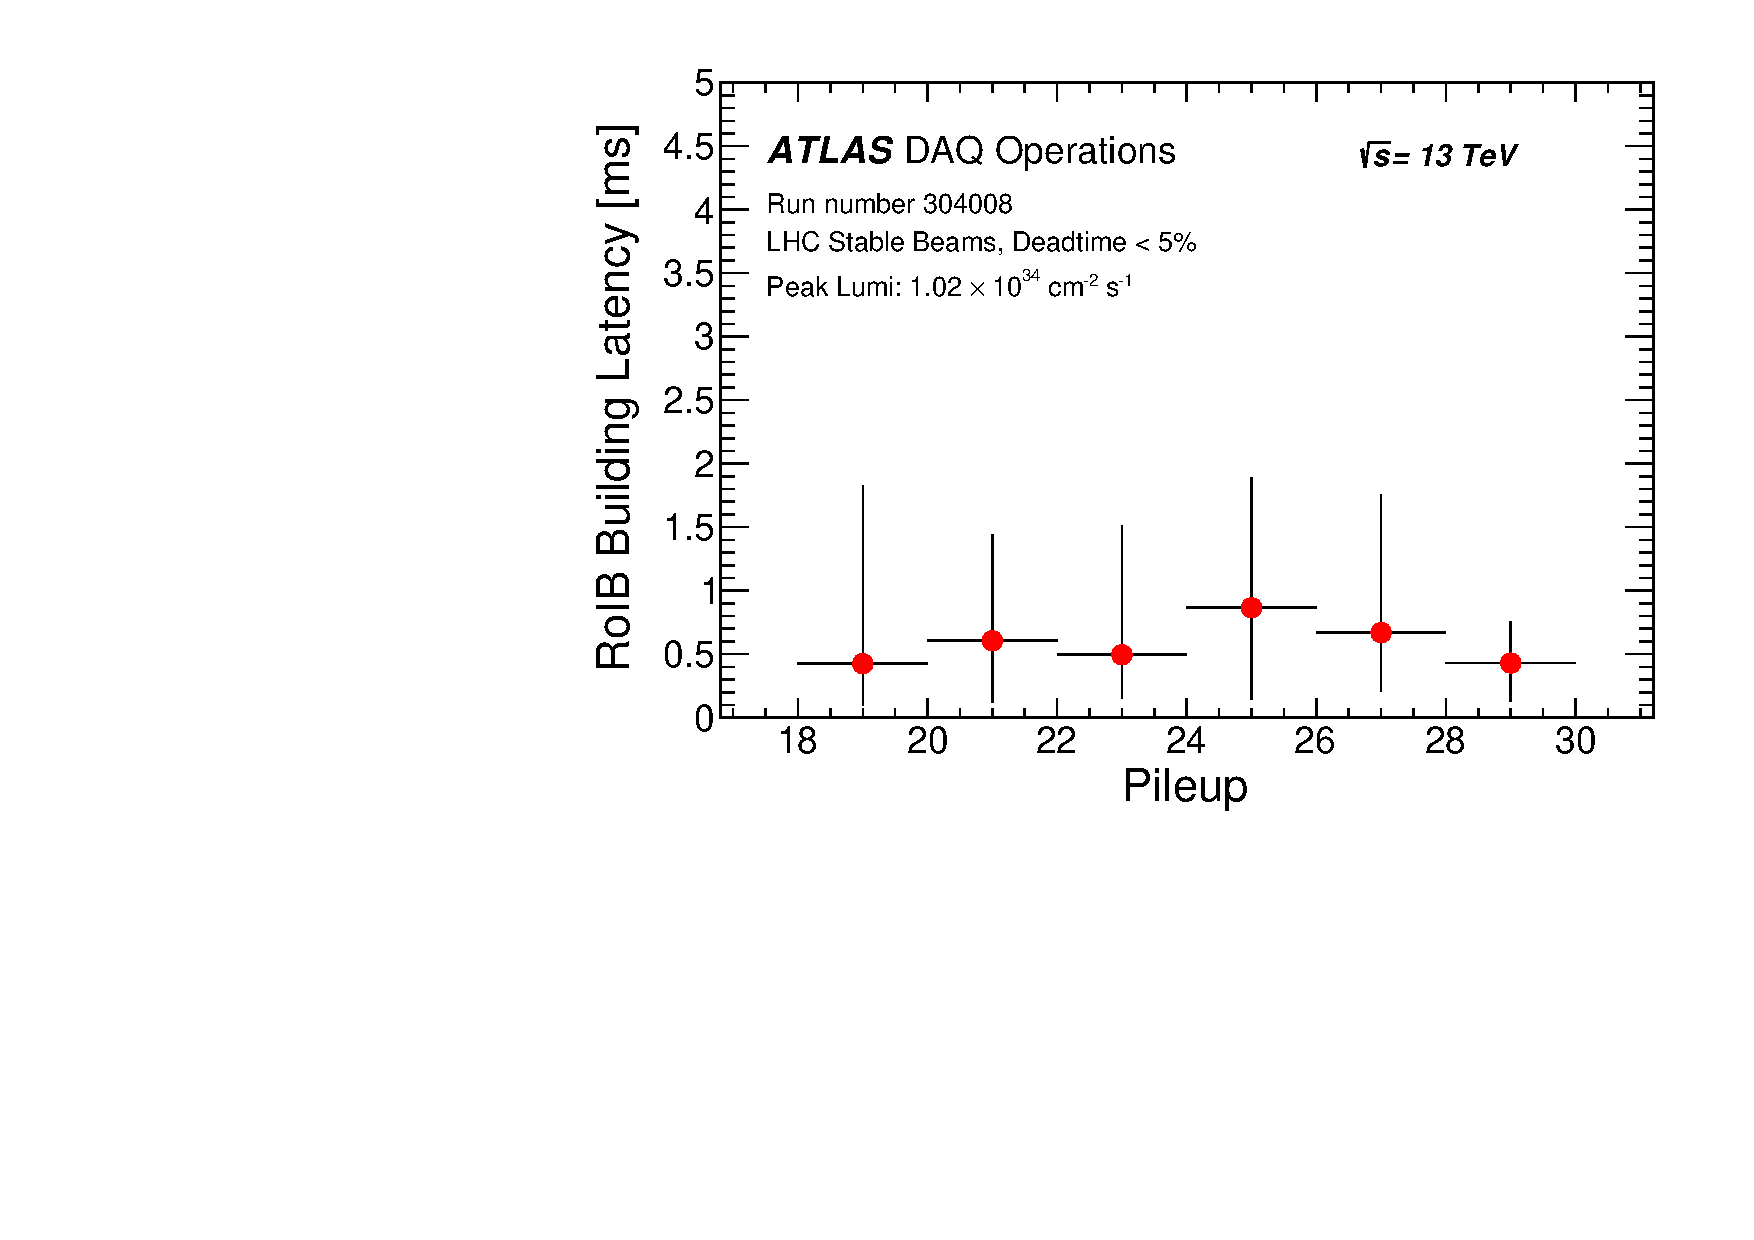
\includegraphics[width=0.95\textwidth]{GrAssym_run_304008_pileup_RoIBbuildtime}
\subcaption{}
\label{fig:roib.perf.buildtime}
\end{subfigure}
\begin{subfigure}[t]{0.48\textwidth}
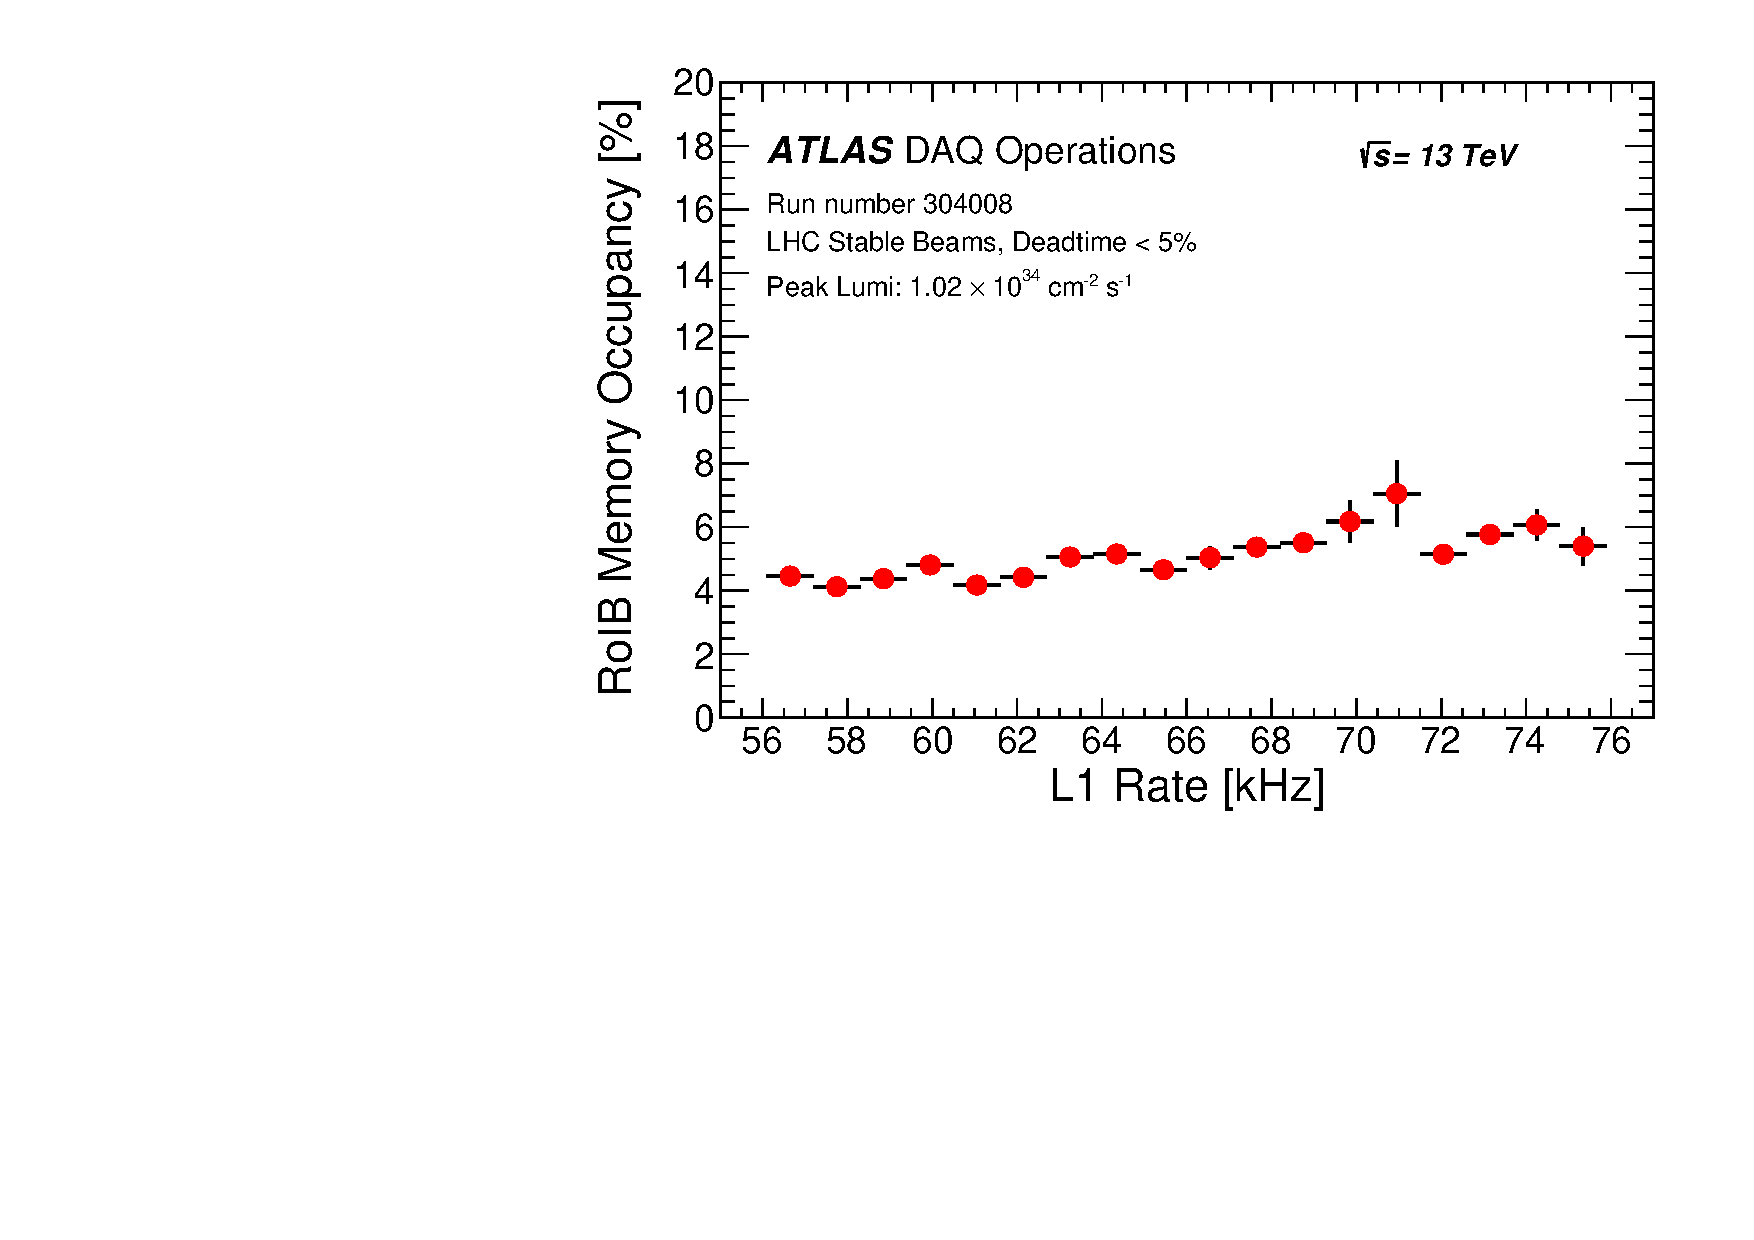
\includegraphics[width=0.95\textwidth]{hProf_run_304008_l1rate_RoIBMemOccup}
\subcaption{}
\label{fig:roib.perf.mem}
\end{subfigure}
\vspace{-0.25cm}
\caption{RoIB performance: RoIB building latency as a function of pileup (left), RoIB memory occupancy as a function of L1 rate (right).}
\label{fig:roib_pileup_l1rate}
\end{figure} 




%% \begin{figure}[t!]
%% \centering
%% \begin{subfigure}[t]{0.48\textwidth}
%% 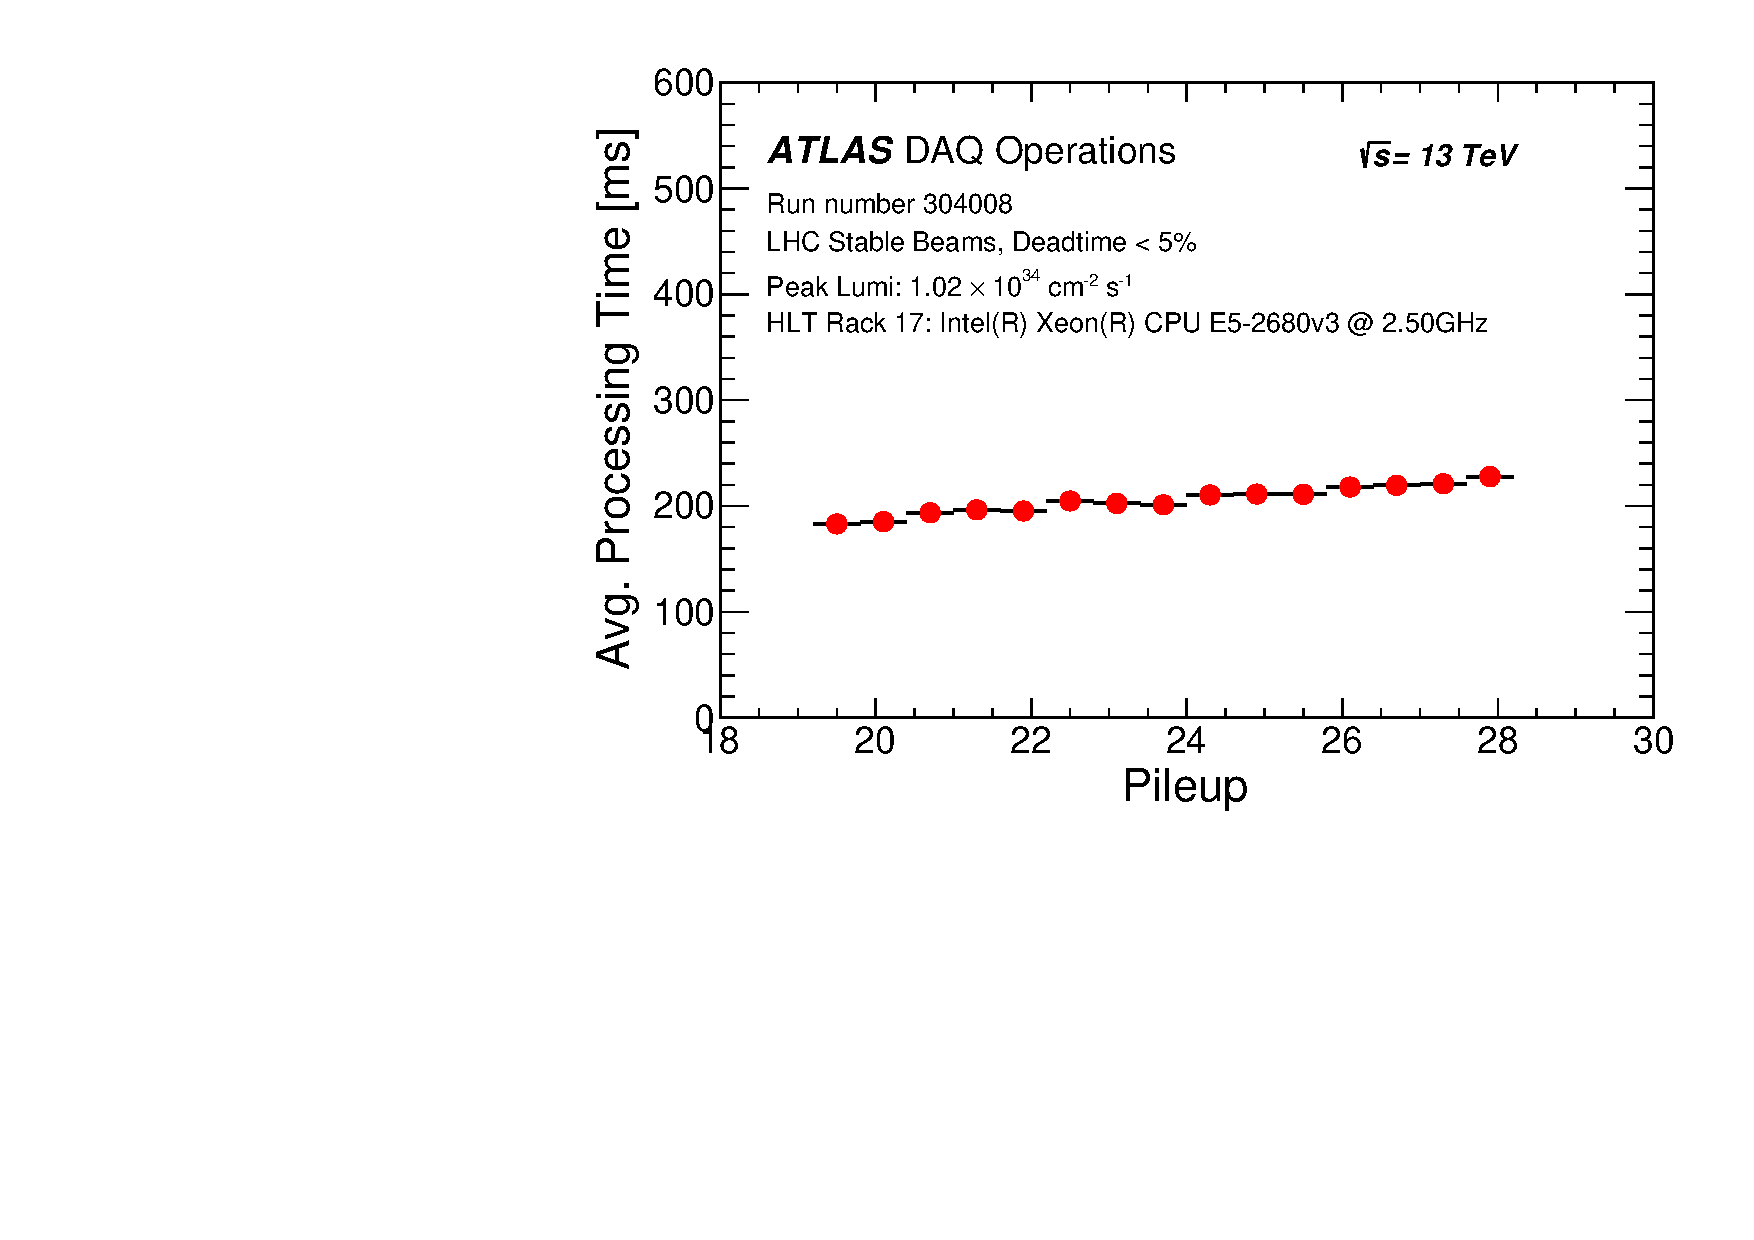
\includegraphics[width=0.95\textwidth]{hProf_run_304008_pileup_AvgProcessingTime}
%% \end{subfigure}
%% \begin{subfigure}[t]{0.48\textwidth}
%% 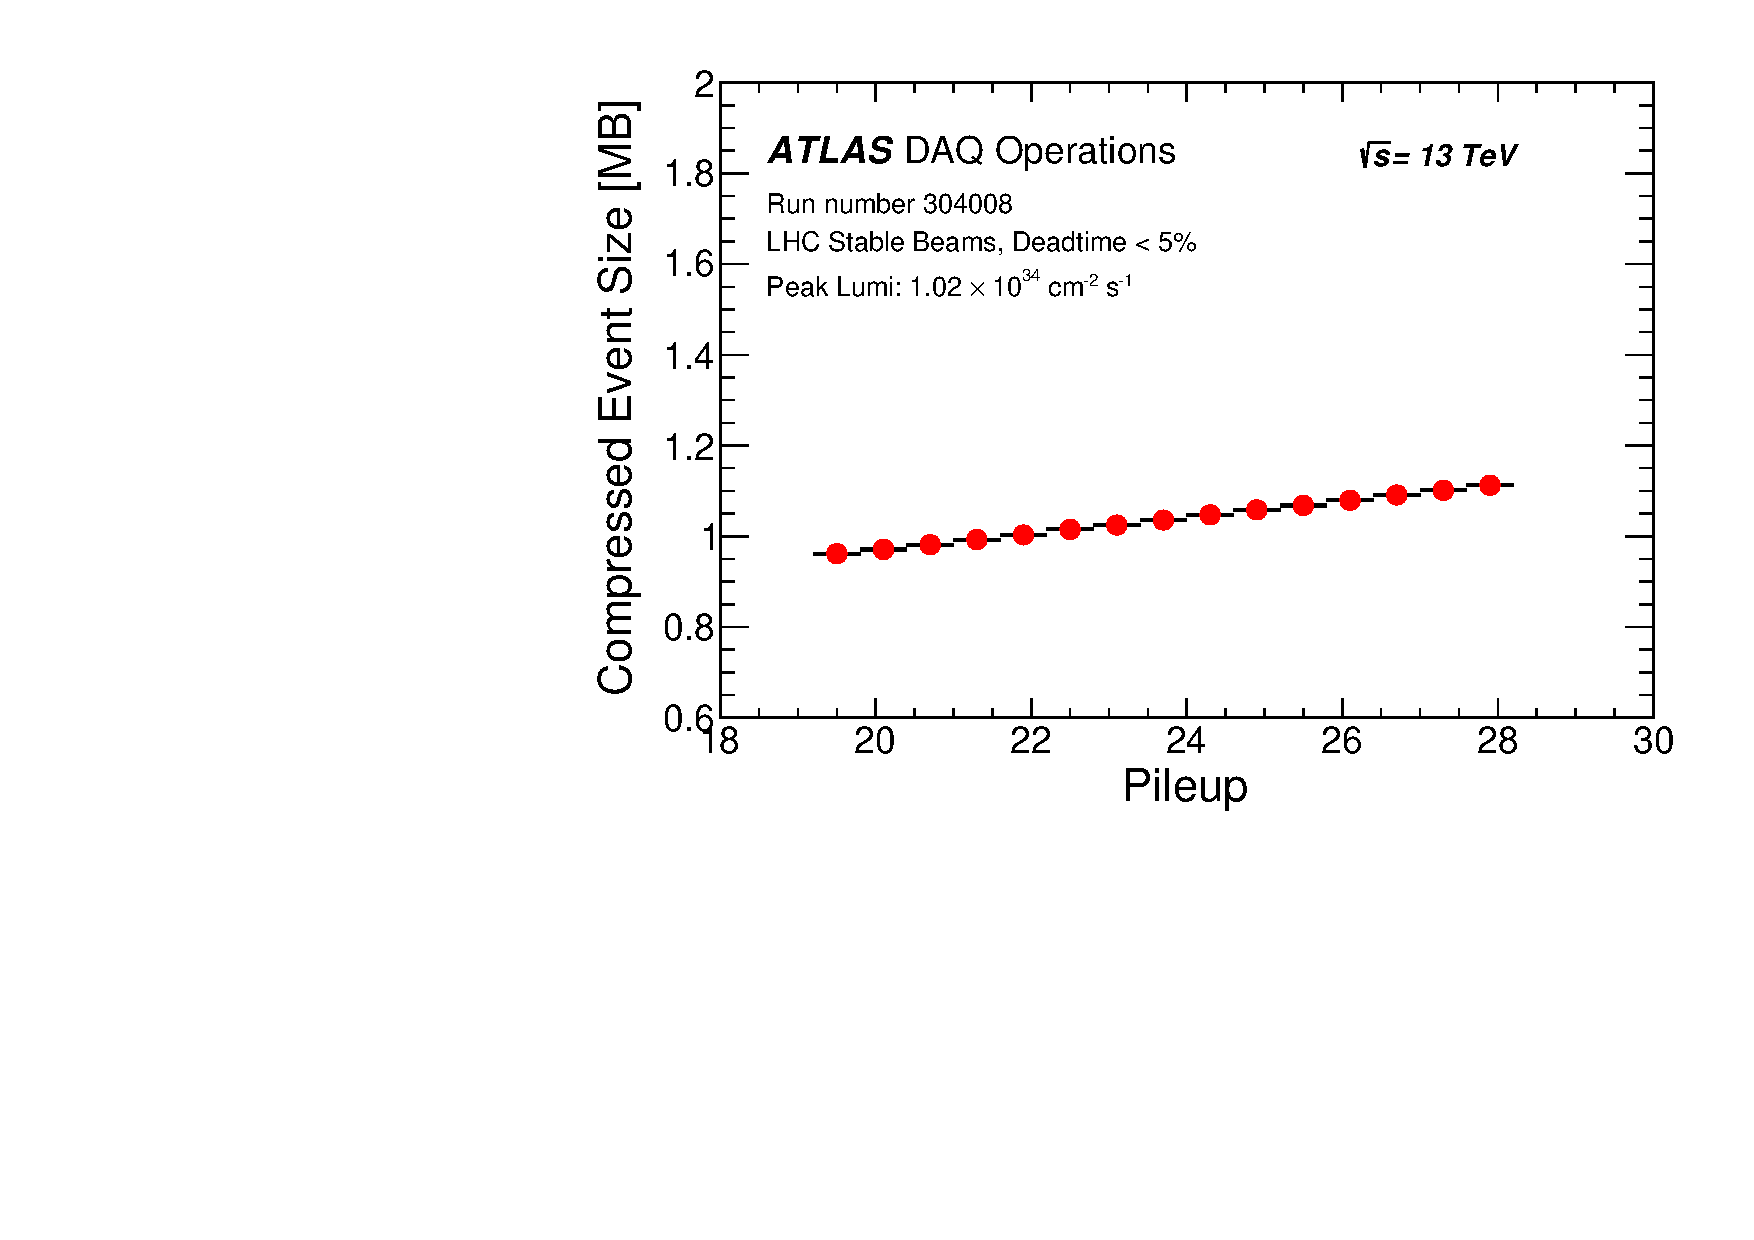
\includegraphics[width=0.95\textwidth]{hProf_run_304008_pileup_EventSize}
%% \end{subfigure}
%% \vspace{-0.25cm}
%% \caption{}
%% \label{fig:roib.perf.proc}
%% \end{figure} 
